\documentclass[main]{subfiles}
\begin{document}

%@@@@@@@@@@@@@@@@@@@@@@@@@@@@@@
% Main Topics: Membrane Potential 04.10.2018
% Lecturer: Valerio Mante
% author: Vanessa Leite - base document from benelot/eth-intro-to-neuroinformatics-summary

\section{Membrane Potential}
\subsection{Introduction}
In the lowest level, the brain process information in each processing unit (neurons) through membrane potential, molecules and ions.

Experiments in visual area of monkeys and cats (V1 recordings) allowed us to know more about the visual system. We now know that the visual system has orientation selectivity and the MT area respond to motion/velocity.

\href{https://www.youtube.com/watch?v=8VdFf3egwfg}{Here} you can see an experiment and hear the neurons firing.

\subsection{Membrane structure}
\begin{itemize}[noitemsep,nolistsep]
	\item The membrane is bilayer and creates an energy barrier.
	\item Ions can not just flow through. Channels and pumps are needed.
	\item ECS: Extra cellular solution.
	\item ICS: Intra cellular solution.
	\item Membrane is built of two types of molecules, charged hydrophilic dipole head-group (outside) and an uncharged, hydrophobic hydrocarbon tail.
	\item It is a phospholipid bilayer.
\end{itemize}

\subsection{Hyperpolarization}
\begin{itemize}[noitemsep,nolistsep]
	\item The extracellular space has potential $V=0\,mV$.
	\item The intracellular space has resting potential $V=-70\,mV$.
\end{itemize}

\subsection{Inputs to neurons, excitatory}
\begin{itemize}[noitemsep,nolistsep]
	\item Inputs to neurons over synapses.
	\item Depolarization, about $V=30\,mV$ presynaptic.
	\item Excitatory current is positive charge, which comes from the extra- to intra-cellular space.
	\item The signal is analog and graded.
	\item On the way to the soma, the intra-cellular current gets reduced by leak current (positive charge) that leaves the intra-cellular space.
	\item From the large depolarization ($V=0\,mV$), about $V=-69.5\,mV$ is the value at the soma.
	\item EPSP (excitatory postsynaptic potential) $0.2$ to $0.4\,mV$.
	\item Spatial and temporal spread of the signal.
	\item $\tau_m$ defines how fast potentials changes.
	\item $\lambda$ defines how far currents travel.
\end{itemize}
\begin{figure}[H]
	\centering
	\scalebox{0.7}{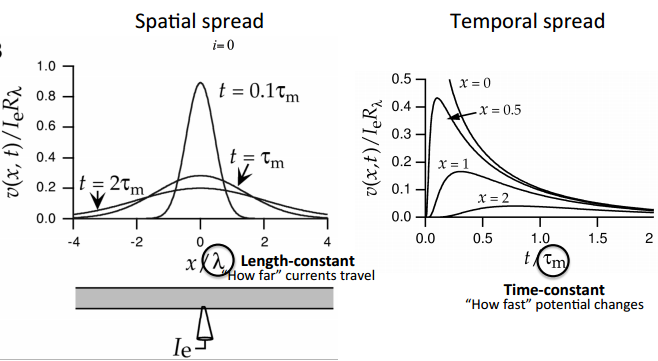
\includegraphics{spatial_temporal_spread.png}}
\end{figure}

\subsection{Chemical synapses}
\begin{figure}[H]
	\centering
	\scalebox{0.7}{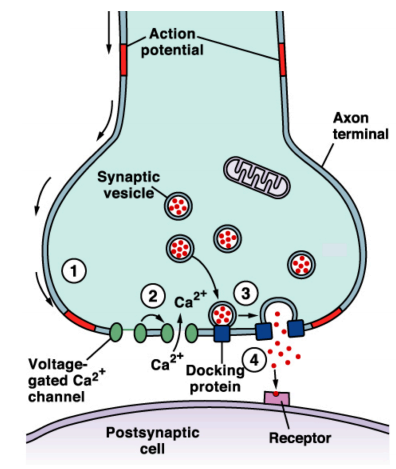
\includegraphics{chemical_synapse.png}}
\end{figure}
\begin{itemize}[noitemsep,nolistsep]
	\item Digital transmission, but can have failures, and graded release.
	\item There can even be synapses directly on the soma or axon.
\end{itemize}

\subsection{Inhibitory post-synaptic potential}
\begin{itemize}[noitemsep,nolistsep]
	\item Depolarization, about $V=30\,mV$ presynaptic.
	\item A large hyperpolarization, $V=-90\,mV$ at postsynaptic dendrite.
	\item Small hyperpolarization at soma, $V=-70.2\,mV$.
\end{itemize}

\subsection{Summation of Inputs}
\begin{itemize}[noitemsep,nolistsep]
	\item Temporal summation, one input after another.
	\item Spatial summation, inputs from different dendrite branches.
	\item Summing up, the threshold is crossed.
	\item Typically 20 to 30 Inputs are needed to go above threshold.
	\item The action potential gets triggered at the beginning of the axon.
	\item The threshold is about $-60\,mV$.
\end{itemize}

\subsection{Action potential}
\begin{itemize}[noitemsep,nolistsep]
	\item Has an active regenerative process.
	\item The duration is about 1 to 2 ms.
	\item All-or-none (digital).
	\item Amplitude gets converted into rate.
	\item Components: Depolarization, overshoot ($>0\,mV$), repolarization/hyperpolarization and a refractory period (back to $-70\,mV$).
	\item Peak about $0.5\,ms$ long, $4.4\,ms$ refractory period.
\end{itemize}
\begin{figure}[H]
	\centering
	\begin{subfigure}[b]{0.5\textwidth}
		\centering
		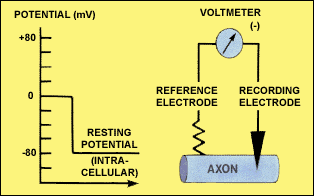
\includegraphics[width=\textwidth]{voltage-source-in-membrane.png}
	\end{subfigure}%
	~
	\begin{subfigure}[b]{0.5\textwidth}
		\centering
		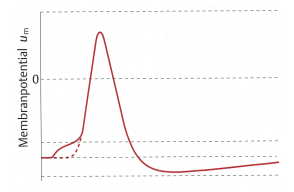
\includegraphics[width=\textwidth]{action_potential_01.png}
	\end{subfigure}
\end{figure}
\begin{figure}[H]
	\centering
	\begin{subfigure}[b]{0.5\textwidth}
		\centering
		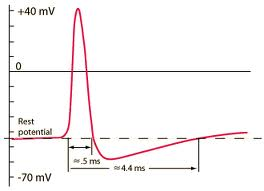
\includegraphics[width=\textwidth]{voltage-source-in-membrane2.png}
	\end{subfigure}%
	~
	\begin{subfigure}[b]{0.5\textwidth}
		\centering
		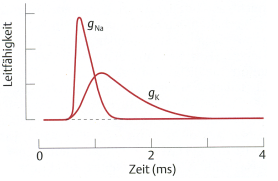
\includegraphics[width=\textwidth]{action_potential_02.png}
	\end{subfigure}
\end{figure}

\subsection{Axon}
\begin{itemize}[noitemsep,nolistsep]
	\item Myelin sheet is often wrapped around the axon.
	\item This makes the white-matter white.
	\item Myelin is an electrical insulator which grants faster propagation.
	\item Less energy is needed with myelinated axons.
	\item The current goes through the node of ranvier (myelin sheath gaps).
\end{itemize}

\subsection{Ionic currents and equilibrium}
\subsubsection{Receptors:}
\begin{itemize}[noitemsep,nolistsep]
	\item Excitatory: AMPA/NDMA, mixed cation, $V(drive) =0\,mV$
	\item Inhibitory: GABA A, chloride (Cl), $V(drive) =-65\,mV$
	\item Inhibitory: GABA B, potassium (K), $V(drive) =-90\,mV$
\end{itemize}
\subsubsection{Action potential:}
\begin{itemize}[noitemsep,nolistsep]
	\item Sodium (Na): $V(drive) = 55\,mV$
	\item Potassium (K); $V(drive) = -90\,mV$
\end{itemize}

\subsubsection{Ion equilibrium}
\textbf{Charge carrier (giant squid axon)}:\\
\begin{tabular}{|l|l|l|l|}
	\hline
	Ion type & Cytoplasm (mM) & Extracellular (mM) & Equilibrium potential (mV)\\\hline
	$K^+$ & 400 & 20 & -75 \\\hline
	$Na^+$ & 50 & 440 & +55\\\hline
	$Cl^-$ & 52 & 560 & -60\\\hline
	$Ca^{2+}$ & 0.0001 & 10 &\\\hline
	Organic anions & 385 & - &\\\hline
\end{tabular}
\begin{figure}[H]
	\centering
	\scalebox{0.5}{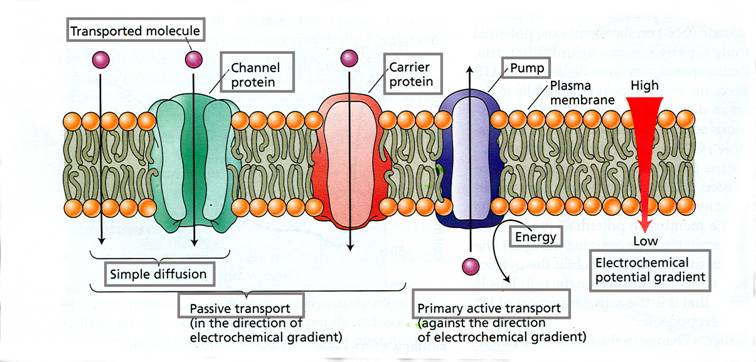
\includegraphics{bilayer-closeup2.png}}
\end{figure}

\subsection{Nernst-Equation}
\subsubsection{Acting forces}
\begin{itemize}[noitemsep,nolistsep]
	\item Ion concentration gradient (diffusion).
	\item Electric potential (electrostatic force).
	\item Both forces are in equilibrium in resting/passive state.
	\item Equilibrium potential can be computed with the Nernst equation.
	\item Neurons have $K^+$, $Na^+$ and $Cl^-$ channels.
	\item $K^+$ permeability is greater than $Na^+$ permeability.
	\item Active $Na^+$-$K^+$ pump creates an ion gradient. The exchange is 2 $K^+$ against 3 $Na^+$ ions.
\end{itemize}

\subsubsection{General equation}
\[E_{ion}= \frac{RT}{zF} \cdot \ln (\frac{[Ion]_{extracellular}}{[Ion]_{intracellular}})\]
\begin{itemize}[noitemsep,nolistsep]
	\item R: Universal gas constant ($8.3144\,\frac{J}{mol \cdot K}$).
	\item T: Absolute temperature (kelvin).
	\item F: Faraday constant ($ 96500\,\frac{C}{mol}$).
	\item z: Number of electrons involved (1 for $K^+$, 2 for $Ca^{2+}$).
	\item One mole has $6.022\cdot10^{23}$ ions, solution is one molar when its concentration is $1\,\frac{mol}{l}$.
\end{itemize}

\subsubsection{Simplified equation}
\begin{itemize}[noitemsep,nolistsep]
	\item Take the temperature as $37\,\degree C$ or $25\,\degree C$.
	\item Replace $\ln$ with $\log$, gives a factor $2.3$.
	\item This gives a factor $60$ respectively $58$ for $\frac{RT}{F}$.
\end{itemize}
\[E_{ion}= \frac{58}{z} \cdot \log_{10} (\frac{[Ion]_{extracellular}}{[Ion]_{intracellular}})\]

\begin{figure}[H]
	\centering
	\begin{subfigure}[b]{0.5\textwidth}
		\centering
		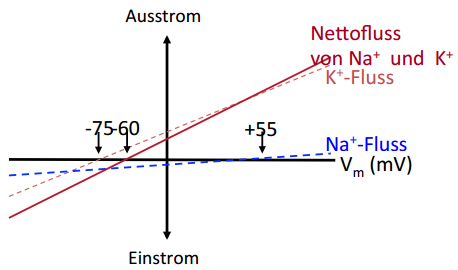
\includegraphics[width=\textwidth]{equilibrium_nernst_01.png}
	\end{subfigure}%
	~
	\begin{subfigure}[b]{0.3\textwidth}
		\centering
		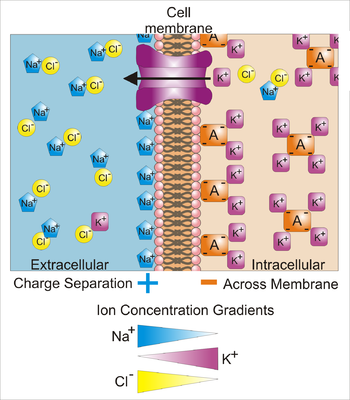
\includegraphics[width=\textwidth]{membrane_potential.png}
	\end{subfigure}
\end{figure}

\subsection{Goldmann-Equation}
\begin{itemize}[noitemsep,nolistsep]
	\item Nernst does not consider multiple ions and permeability.
	\item Goldmann describes membrane potential, with multiple ions and permeability.
	\item Assumes ion flux obeys Nernst/Planck equation.
	\item Assumes ions move across membrane independently, without interaction.
	\item Equilibrium: $P_K:P_{Na}:P_{Cl}$ is $1:0.04:0.45$.
	\item Action potential: $P_K:P_{Na}:P_{Cl}$ is $1:20:0.45$.
	\item $V_m$: Membrane potential.
	\item $P$: Membrane permeability.
	\item $[A^x]$: Ion concentration.
\end{itemize}

\[V_m = \frac{RT}{F} ln(\frac{P_K[K^+]_{out} + P_{Na}[Na^+]_{out} + P_{Cl}[Cl^{-}]_{in}}{P_K[K^+]_{in} + P_{Na}[Na^+]_{in} + P_{Cl}[Cl^{-}]_{out}})\]



\end{document}
